% Created 2014-11-20 Thu 21:57
\documentclass[9pt,b5paper]{article}
\usepackage{graphicx}
\usepackage{xcolor}
\usepackage{xeCJK}
\usepackage{longtable}
\usepackage{float}
\usepackage{textcomp}
\usepackage{geometry}
\geometry{left=0cm,right=0cm,top=0cm,bottom=0cm}
\usepackage{multirow}
\usepackage{multicol}
\usepackage{listings}
\usepackage{algorithm}
\usepackage{algorithmic}
\usepackage{latexsym}
\usepackage{natbib}
\usepackage{fancyhdr}
\usepackage[xetex,colorlinks=true,CJKbookmarks=true,linkcolor=blue,urlcolor=blue,menucolor=blue]{hyperref}


\lstset{language=c++,numbers=left,numberstyle=\tiny,basicstyle=\ttfamily\small,tabsize=4,frame=none,escapeinside=``,extendedchars=false,keywordstyle=\color{blue!70},commentstyle=\color{red!55!green!55!blue!55!},rulesepcolor=\color{red!20!green!20!blue!20!}}
\author{Heyan Huang}
\date{\today}
\title{Fall 2014 CS580 MIDI Command Controller Interface}
\hypersetup{
  pdfkeywords={},
  pdfsubject={},
  pdfcreator={Emacs 24.3.1 (Org mode 8.2.7c)}}
\begin{document}

\maketitle
\tableofcontents


\section{11/21/2014 Update}
\label{sec-1}
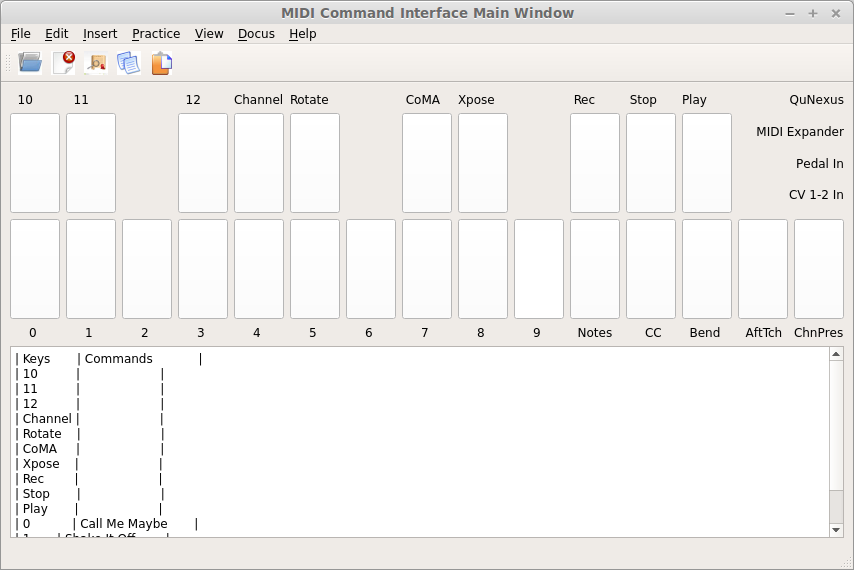
\includegraphics[width=.9\linewidth]{./pic/2014-11-20_21:52:19.png}

\section{main functionality}
\label{sec-2}
\subsection{Read data from MIDI}
\label{sec-2-1}
\begin{itemize}
\item Use the MIDI Controller as a speical Controller that can be operated to play specific songs sequence, or do some specific work.
\item play specific sequence may be the work for keys 0-9, and 10-12, how about other 20 keys? Do they require specific work to be done?
\end{itemize}

\subsection{Write data back to MIDI}
\label{sec-2-2}
\begin{itemize}
\item When a key was pushed, the specific Controller key's LED is supposed to be on to indicate the operation.
\item Trick about the LED to be continuously on is that when a key is pressed, that is 1 byte that indicates the "Duration" of the key press, I may need to 
\begin{itemize}
\item try to set this byte to be a large value, (1 byte, 2$^{\text{8}}$ = 256, it has limits!)
\item or continuously reset is to be that large value;
\item or continuously write this key to be pressed data back to MIDI with time intervals
\end{itemize}
\end{itemize}

\section{Programming Language}
\label{sec-3}
\subsection{Qt}
\label{sec-3-1}
\begin{itemize}
\item the worries that I have by using Qt is that if Qt has the capability to handle the MIDI-Linux connection problems.
\item And also Qt-to-Audio (linux) connection things as well. Should it be Qt, or as far as I can set it to work in Linux, just let it be that way then?
\end{itemize}
\subsection{c++}
\label{sec-3-2}
\begin{itemize}
\item I believe C++ is the most widely used Language used by those midi sequencer softwares, so I have no better choice than c++ right now.
\end{itemize}

\section{Interface Design}
\label{sec-4}
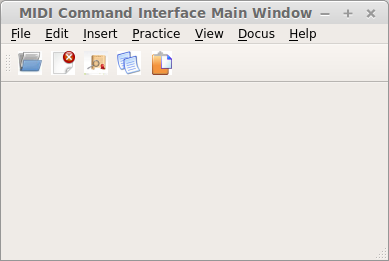
\includegraphics[width=.9\linewidth]{./menu.png}

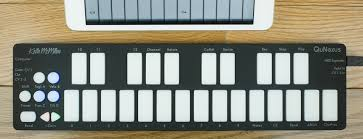
\includegraphics[width=.9\linewidth]{./midi.jpg}

\section{Midi keys and corresponded operations}
\label{sec-5}
\begin{table}[htb]
\caption{midi keys and corresponded operations}
\centering
\begin{tabular}{ll}
\hline
Keys & Commands\\
\hline
10 & \\
11 & \\
12 & \\
channel & \\
Rotate & \\
CoMA & \\
Xpose & \\
Rec & \\
Stop & \\
Play & \\
\hline
0 & Call Me Maybe\\
1 & Shake It Off\\
2 & All About That Bass\\
3 & \ldots{}\\
4 & \\
5 & \\
6 & \\
7 & \\
8 & \\
9 & \\
\hline
Notes: & \\
CC & \\
Bend & \\
AftTch & \\
ChnPres & \\
\hline
Togl A & \\
Velo B & \\
Preset & \\
Pres C & \\
Tilt D & \\
Bend & \\
Oct- & \\
Oct+ & \\
\hline
\end{tabular}
\end{table}

\section{Interface Guide}
\label{sec-6}
\begin{itemize}
\item Give text instructions on how to use the Interface, and what are the corresponded operations by press specific keys.
\item Like list the above table in the Interface Guide text area.
\end{itemize}
% Emacs 24.3.1 (Org mode 8.2.7c)
\end{document}